%For pdftex and Latex Fonts
%\usepackage{crimson} % Crimson Font
%\usepackage{CormorantGaramond} % Cormorant Garamond
%\usepackage{ebgaramond} % EB Garamond
%\usepackage[sfdefault]{FiraSans} % Fira Sans
%\usepackage[default]{lato} % Lato
%\usepackage[sfdefault]{noto} % Noto
%\usepackage[default,osfigures,scale=0.95]{opensans} % Open Sans
\usepackage[sfdefault]{roboto} % Roboto Font
%\usepackage[default]{sourcesanspro} % Souce Sans Pro
%\usepackage[default,light]{sourceserifpro} % Source Serif Pro
\usepackage[T1]{fontenc}

%Load Other Packages
\usepackage{calc}  
\usepackage{enumitem}
\usepackage{setspace}

%Set Header and Footers
\usepackage{fancyhdr}
\pagestyle{fancy}
\fancyhf{}
\rhead{Share\LaTeX}
\lhead{Guides and tutorials}
\rfoot{Page \thepage}

%% For Fancy Header and Footer Lines
%\renewcommand{\headrulewidth}{2pt}
%\renewcommand{\footrulewidth}{1pt}

%Adding & Formatting Title Page
\usepackage{titling}
\renewcommand\maketitlehooka{\null\mbox{}\vfill}
\pretitle{%
  \begin{center}
  \bfseries
  \color{gray}
  \LARGE
  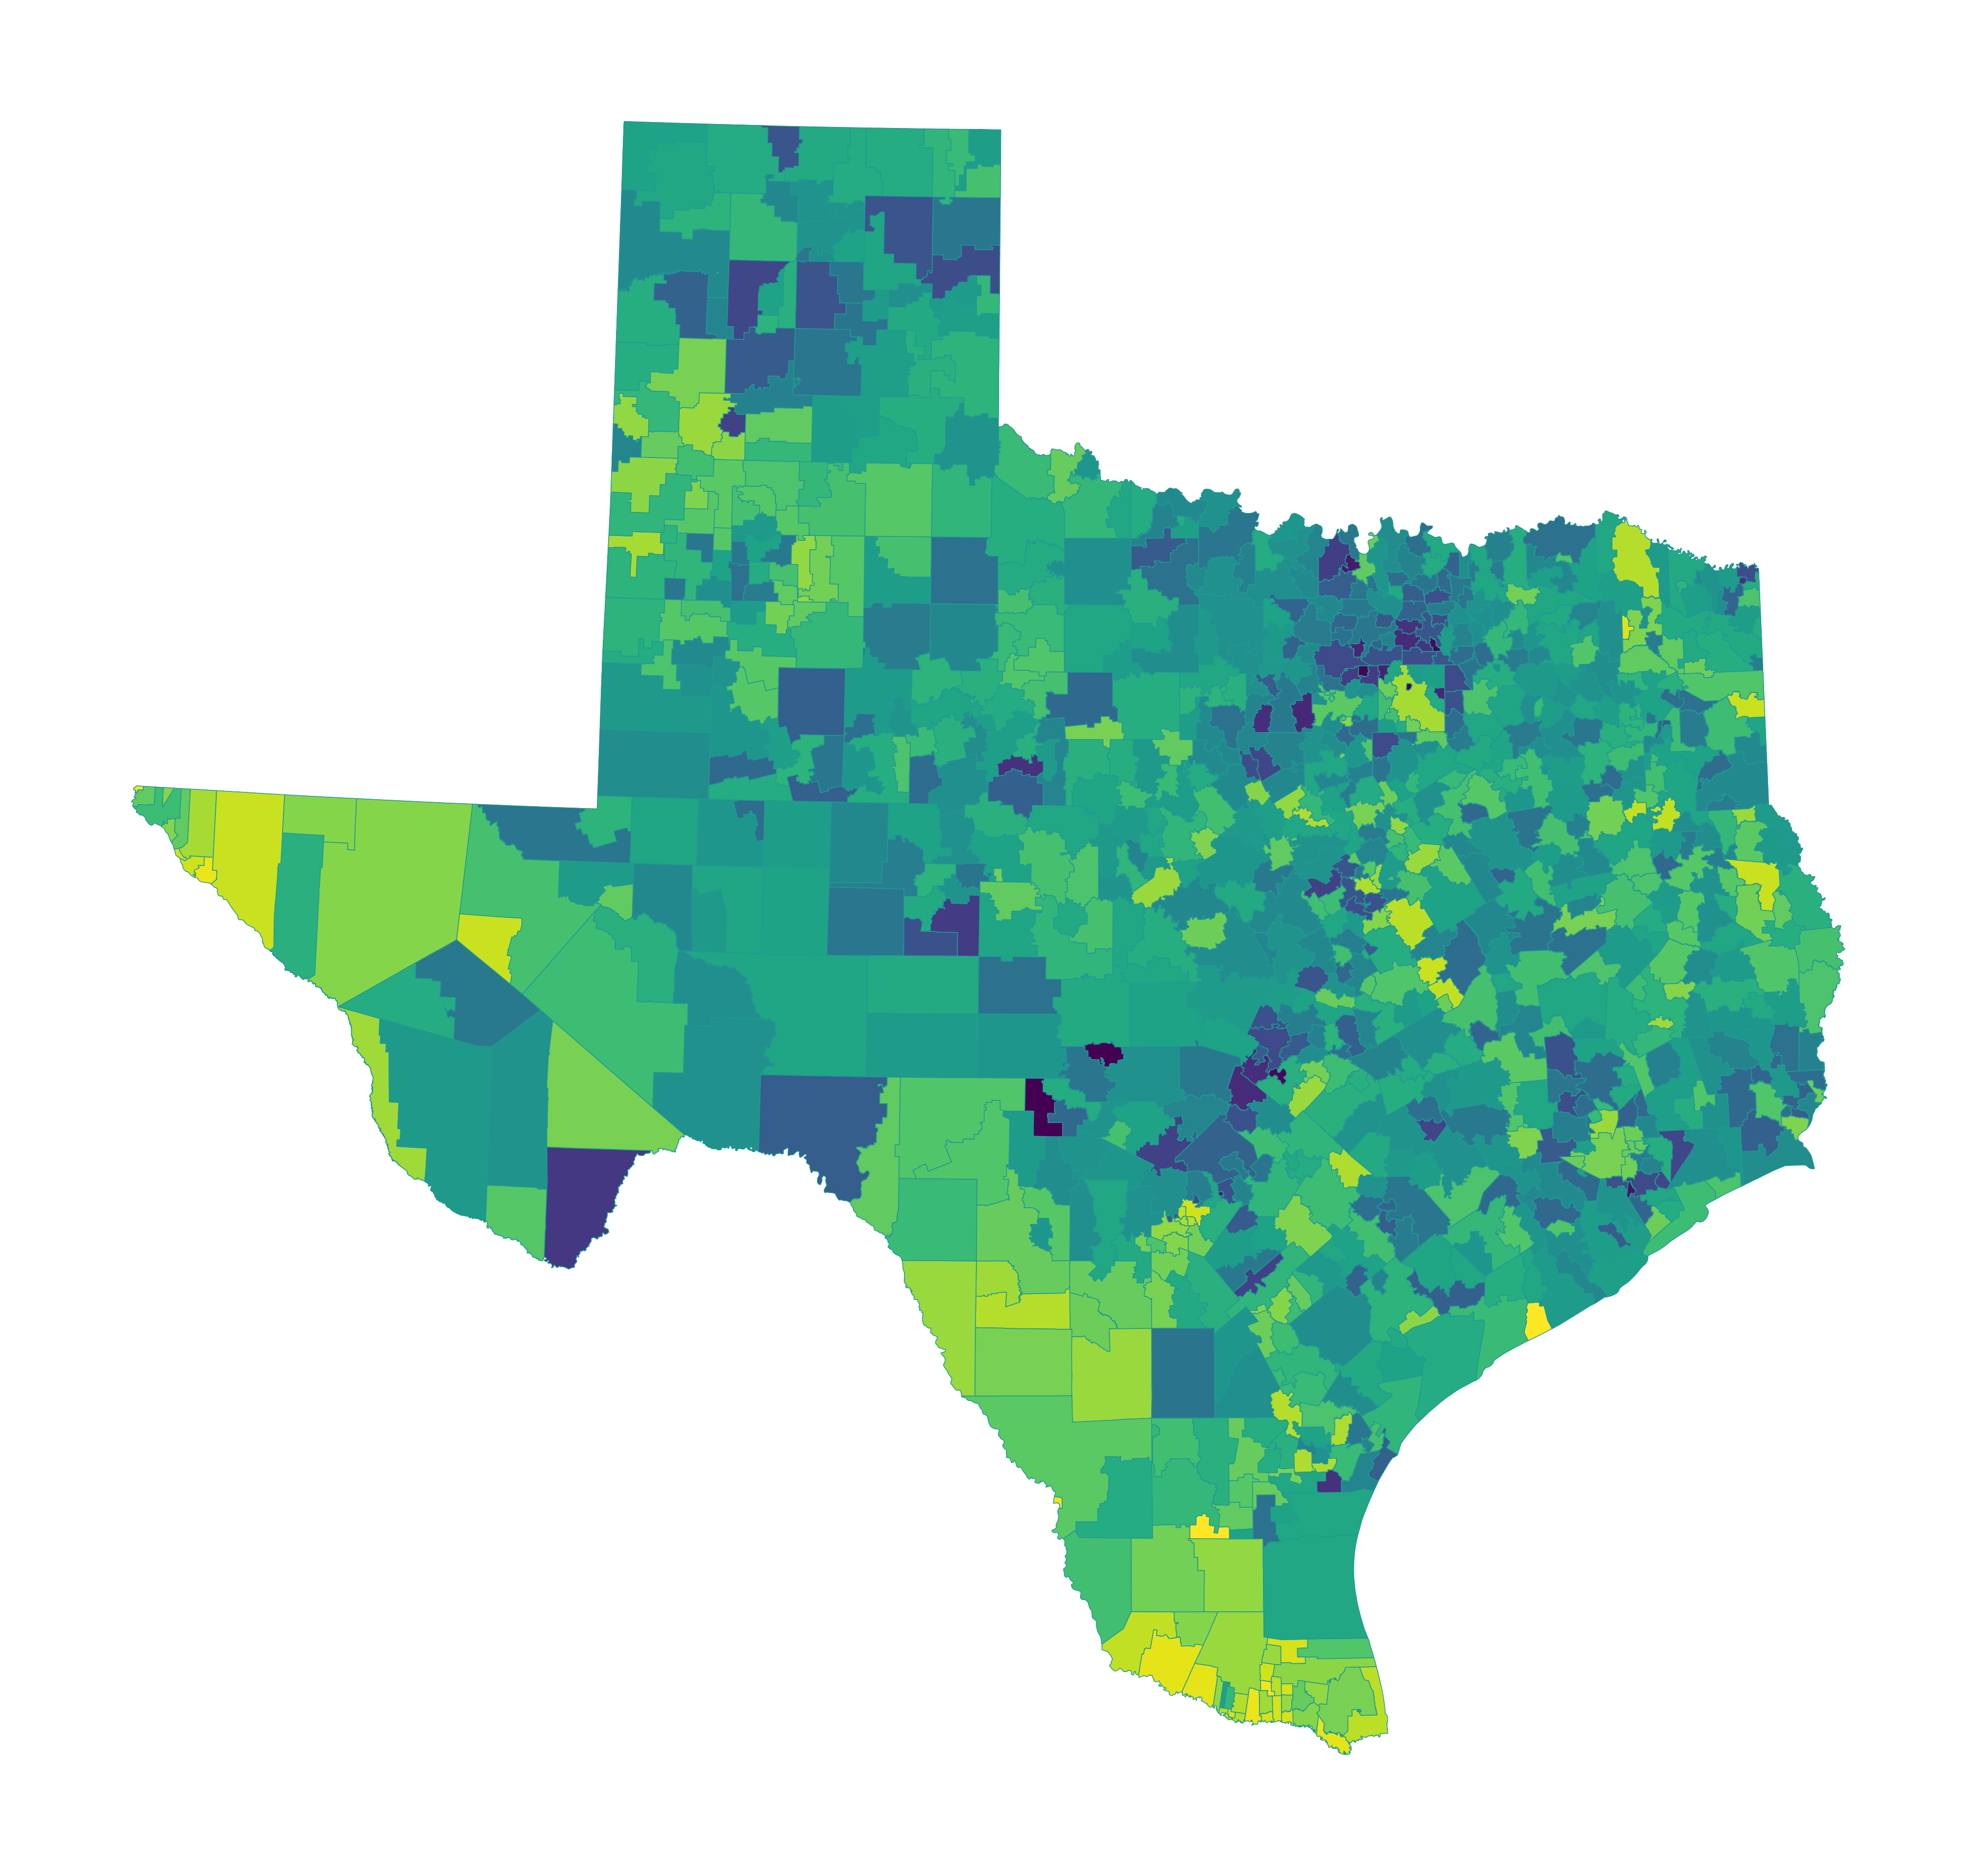
\includegraphics[width=12cm]{images/Texas.png}\\[\bigskipamount]}
  
\includegraphics[width=12cm]{images/LBJ Logos/Text_FullCenter2.png}\\[\bigskipamount]}
\posttitle{\subtitle{center}\end{center}}
\renewcommand\maketitlehookd{\vfill\null}

%General Text Formatting
\color{textgray3} %Main Text Color

\renewcommand{\baselinestretch}{1.3} %Lineh
\widowpenalty=1000
\clubpenalty=1000

%Section Styling
\sectionfont{\LARGE\color{blue}}
\subsectionfont{\Large\color{gray}}
\subsubsectionfont{\large\bfseries\color{textgray1}}


%Adjust Figure Position, Width, & Wrap
\usepackage{float}
\let\origfigure\figure
\let\endorigfigure\endfigure
\renewenvironment{figure}[1][2] {
    \expandafter\origfigure\expandafter[H]
} {
    \endorigfigure
}
\usepackage{graphicx}
\setkeys{Gin}{width=.9\linewidth}

%Section Paragraph Formatting 
\usepackage{sectsty}
\usepackage{booktabs}
\usepackage{wrapfig}
\usepackage{scrextend}
\changefontsizes{10pt}

%Set Document Colors
\usepackage[table]{xcolor}
\definecolor{gray}{rgb}{.302,.302,.302}
\definecolor{blue}{rgb}{.365, .647, .855}
\definecolor{orange}{rgb}{.98,.643,.227}
\definecolor{green}{rgb}{.376,.741,.408}
\definecolor{pink}{rgb}{.945,.486,.69}
\definecolor{brown}{rgb}{.698,.569,.184}
\definecolor{purple}{rgb}{.698,.463,.698}
\definecolor{yellow}{rgb}{.871,.812,.247}
\definecolor{red}{rgb}{.945,.345,.329}
\definecolor{textgray1}{rgb}{.40,.431,.459} % HEX #282b2d
\definecolor{textgray2}{rgb}{.38,.38,.38} % HEX #262626
\definecolor{textgray3}{rgb}{.282,.282,.282} % HEX #1c1c1c
\color{textgray3}
